\section{Knapsack Problem - Problem plecakowy}
Problem plecakowy jest zagadnieniem optymailzacyjnym. Problem ten swoją nazwę wziął z analogii do rzeczywistego problemu pakowania plecaka. Rozwiązując ten problem zarówno w praktyce jak i teorii trzeba zachować reguły określające ładowność plecaka dotyczące objętości i nośności plecaka. Knapsack Problem zaczął być intensywnie badany po pionierskiej pracy Dantziga\cite{DantzigArticle} w późnych latach 50 XX wieku. Znalazł on natychmiast zastosowanie w przemyśle oraz w zarządzaniu finansami. Z teoretycznego punktu widzenia, problem plecakowy często występuję jako relaksacja róznorodnych problemów programowania całkowitego\cite{PisingerThesis}.
\subsection{Zastosowanie}
Problem plecakowy stosowany jest nie tylko w sytuacji wynikającej bezpośrednio z nazwy. Znajduje on zastosowanie w wielu dziedzinach życia oraz nauki. Diffi i Helman\cite{DiffieHelmanArticle} w 1976 roku oraz Merkle i Helman\cite{MerkleHelmanArticle} w 1978 roku zaproponowali problem plecakowy jako podstawę do enkrypcji kluczy prywatnych. Jednakże podejście to w latach późniejszych zostało złamane przez środowisko kryptograficzne i jego miejsce zajęły bardziej odporne algorytmy.

"Knapsack problem" jest stosowany również podczas załadunku kontenerów służacych do przewozu materiałów drogą morską. Ładowność oraz gabaryty ładowanych elementów są ograniczane przez budowę i wytrzymałość kontenera.

Problem ten stosowany jest również w dziedzinie finansów. Jest on podstawowym narzędziem do optymalizacji portfela inwestycyjnego. Poprzez uogólnienie i modyfikacje problemu plecakowego zjawiska ekonomiczne mogą być modelowane z większą dokładnością. Przykładowo możliwe jest zakupienie 0, 1, 2 lub więcej akcji inwestycyjnych, a zakup kolejnych akcji może przynieść obniżenie przychodu.

Wiele problemów związanych z planowaniem może być przyrównana do problemu plecakowego gdzie czas wykonywania operacji na maszynie jest zasobem deficytowym. Jest on szczególnie uwydatniony gdy od aktywności maszyny zależy kapitał przedsiębiorstwa. Poprzez rozwiązanie problemu plecakowego możliwe jest przewidzenie zapotrzebowania na materiały podaczas procesu tak aby warunki zamówinia zostały spełnione\cite{BartholdiChapter}.

Kolejnym zagadnieniem wynikającym z problemu plecakowego jest problem optymalnego rozkroju, zostanie on przedstawiony w rozdziale \cref{sec:cuttingStockProblem}.
\subsection{Różnorodność problemu plecakowego}
Wszystkie elementy z rodziny tego problemu wymagają pewnego zestawu elementów które mogą zostać wybrane w taki sposób że zysk zostanie zmaksymalizowany, a pojemość placaka lub plecaków nie zostanie przekroczona. Wszystkie typy problemu należą do rodziny problemów $NP-trudnych$ co oznacza, że raczej nispotykane jest rozwiązanie problemu z użyciem algorytmów wielomianowych. Możliwe są różne warinaty problemu zależna od rozmieszczenia elementów oraz ilości plecaków\cite{PisingerThesis}:
\begin{itemize}
  \item \textit{Problem plecakowy 0-1} - każdy element może być wybrany tylko raz. Problem polega na wyborze $n$ elementów dla których suma profitów $p_j$ jest największa, bez konieczności osiągnięcia całkowitej pojemności $c$. Może być sformułowany jako problem maksymalizacji:
  \begin{equation}\label{01Knapsack}
    \begin{aligned}
      & \textrm{maksymalizacja} & & \sum_{j=1}^n p_jx_j, \\
      & \textrm{w odniesieniu do} & & \sum_{j=1}^n w_jx_j \le c, \\
      &&& x_j \in \{0,1\},& j = 1,\dots,n
    \end{aligned}
  \end{equation}
  gdzie $x_j$ jest wartością binarną. Jeżeli $x_j = 1$ wtedy $j$-ty element powinien znaleźć się w plecaku, w innym przypadku $x_j = 0$.
  \item \textit{Ograniczony problem plecakowy} - każdy element może być wybrany ograniczoną ilość razy. Zmianą w obecnym problemie względem problemu 0-1 jest ograniczona $m_j$ ilość elementów $j$:
  \begin{equation}\label{boundedKnapsack}
    \begin{aligned}
      & \textrm{maksymalizacja} & & \sum_{j=1}^n p_jx_j, \\
      & \textrm{w odniesieniu do} & & \sum_{j=1}^n w_jx_j \le c, \\
      &&& x_j \in \{0,1\dots,m_j\},& j = 1,\dots,n
    \end{aligned}
  \end{equation}
  \item \textit{Nieograniczony problem plecakowy} - jest rozszerzeniem problemu ograniczonego o nielimitowaną liczbę dostępnych elementów:
  \begin{equation}\label{unboundedKnapsack}
    \begin{aligned}
      & \textrm{maksymalizacja} & & \sum_{j=1}^n p_jx_j, \\
      & \textrm{w odniesieniu do} & & \sum_{j=1}^n w_jx_j \le c, \\
      &&& x_j \in \mathbb{N}_0,& j = 1,\dots,n
    \end{aligned}
  \end{equation}
  Każda zmienna $x_j$ w metodzie niograniczonej zostanie ograniczona poprzez pojemność $c$, gdy waga każdego z elementów jest równa przynajmniej jeden. W ogólnym przypadku transformacja problemu nieograniczonego w ograniczony nie przynosi korzyści
  \item \textit{Problem plecakowy wielokrotnego wyboru} - elementy powinny być wybierane z klas rozłącznych. Problem ten jest generalizacją problemu 0-1. Możliwy jest wybór dokładnie jednego elementu $j$ z każdej grupy $N_i$, $i=1,\dots,k$:
  \begin{equation}\label{multichoiceKnapsack}
    \begin{aligned}
      & \textrm{maksymalizacja} & & \sum_{i=1}^k \sum_{j \in N_i} p_{ij}x_{ij}, \\
      & \textrm{w odniesieniu do} & & \sum_{i=1}^k \sum_{j \in N_i} w_{ij}x_{ij} \le c, \\
      &&& \sum_{j \in N_i} x_{ij} = 1, & i =1,\dots,k, \\
      &&& x_j \in\{0,1\},& i = 1,\dots,k, \quad j \in N_i.
    \end{aligned}
  \end{equation}
  Zmienna binarna $x_{ij} = 1$ określa że $j$-ty element został wybrany z $i$-tej grupy. Ograniczenie $\sum_{j \in N_i} x_{ij} = 1, \quad i =1,\dots,k$ wymusza wybór dokładnie jednego elementu z każdej grupy.
  \item \textit{Wielokrotny problem plecakowy} - mozliwość wypełnienia wielu pleckaków. Jeśli jest możliwość załadowania $n$ elmentów do $m$ pleckaów o róznych pojemnościahc $c_i$ w taki sposób że zysk będzie jak największy:
  \begin{equation}\label{multiKnapsack}
    \begin{aligned}
      & \textrm{maksymalizacja} & & \sum_{i=1}^k \sum_{j \in N_i} p_{ij}x_{ij}, \\
      & \textrm{w odniesieniu do} & & \sum_{j=1}^n  w_jx_{ij} \le c_i, & i =1,\dots,m \\
      &&& \sum_{j \in N_i} x_{ij} \le 1, & i =1,\dots,k, \\
      &&& x_j \in\{0,1\},& i = 1,\dots,m, \quad j =1,\dots,n.
    \end{aligned}
  \end{equation}
  Zmienna $x_{ij} = 1$ określa że $j$-ty element powinien zostać umiesczony w $i$-tym plecaku, podczas gdy ogranicznie $\sum_{j=1}^n  w_{ij}x_{ij} \le c_i$ zapewnia że restrykcja dotycząca pojemności plecaka zostanie zachowana. Ogranicznie $\sum_{j \in N_i} x_{ij} \le 1$ zapewnia że każdy element zostanie wybrany tylko raz.
  \item \textit{Bin-packing problem} - bardzo często spotykana wersja problemu plecakowego/ Problem ten polega na umieszczeniu $n$ elementów w jak najmniejszej liczbie opakowań:
  \begin{equation}\label{binPacking}
    \begin{aligned}
      & \textrm{maksymalizacja} & & \sum_{i=1}^n y_i \\
      & \textrm{w odniesieniu do} & & \sum_{j=1}^n w_jx_{ij} \le cy_i, & i=1,\dots,n, \\
      &&& \sum_{i=1}^n x_{ij} = 1, & j=1,\dots,n, \\
      &&& y_i \in \{0,1\}, & i=1,\dots,n, \\
      &&& x_{ij} \in \{0,1\} & i=1,\dots,m, \quad j = 1,\dots,n,
    \end{aligned}
  \end{equation}
  gdzie $y_i$ określa czy $i$-te opakowanie zostało użyte, a $x_{ij}$ stanowi czy $j$-ty element powinen zostać umieszcozny w $i$-tym opakowaniu
  \item \textit{Welokrotnie ograniczony problem plecakowy} - najbardziej ogólny typ który jest problemem programowania całkowitego z dodatnimi współczynnikami:
  \begin{equation}\label{generalKnapsack}
    \begin{aligned}
      & \textrm{maksymalizacja} & & \sum_{j=1}^n p_jx_j, \\
      & \textrm{w odniesieniu do} & & \sum_{j=1}^n w_jx_j \le c_i, & i=1,\dots,m, \\
      &&& x_j \in \mathbb{N}_0, & j = 1,\dots,n.
    \end{aligned}
  \end{equation}
\end{itemize}

\subsection{Możliwe rozwiązania}

Problem plecakowy należy do grupy problemów $\mathcal{NP}$-Trudnych. Rozwiązanie problemów z tej grupy jest co najmniej tak trudne, jak rozwiązanie każdego problemu z całej klasy $\mathcal{NP}$. Problem $\mathcal{NP}$-Trudny to problem obliczeniowy dla którego znalezienie rozwiązania problemu nie jest możliwe z wielomianową złożonościa obliczeniową. Problemy $\mathcal{NP}$-Trudne obejmują zarówno problemy decyzyjne jak również problemy przeszukiwania czy też problemy optymalizacyjne.

Rozwiązanie problemu plecakowego jest możliwe przy użyciu różnych metod:
\begin{itemize}
  \item \textit{Metoda podziału i ograniczeń} - Metoda ta często jest stosowana do problemu plecakowego od momentu gdy Kolesar \cite{KolesarArticle} zaprezentował pierwszy algorytm w 1967 roku.
  \item \textit{Programownaie dynamiczne} - Gdy zostaną dodane warunki brzegowe wtedy algorytm ten staje się "zaawansowaną" formą metody podziału i ograniczeń.
  \item \textit{Relaksacja przestrzeni stanów} - relaksacja programowani dynamicznego gdzie współczynniki są skalowane przez pewną stałą wartość.
\end{itemize}

\subsubsection{Metoda podziału i ograniczeń}
Algorytm ten polega na wypisaniu wszystkich możliwych rozwiązań używając struktury drzewiastej. Algorytm przechodzi kolejno po gałęziach drzewa które reprezentują podzbiory rozwiązania. Każda gałąź jest sprawdzana zadanymi warunkami brzegowymi i jest odrzucana jeśli nie poprawi rozwiąznaia. Przedstawione zostanie rozwiązanie nieograniczonego problemu plecakowego (\cref{unboundedKnapsack}) \cite{ChvatalBook}. Współczynniki $w_1,\dots,w_m$, $p_1, \dots, p_m$ oraz $c$ są nieujemne. Stosunek $p_j/w_j$ jest wartością jednej jednostki długości $j$-tego elementu. Stosunek ten jest \textit{wydajnością} zmiennej $x_j$. Pierwszym krokiem algorytmu jest posortowanie zmiennych w porządku malęjącym względem wydajności:
\begin{equation} \label{eq:BBeff}
  p_1/w_1 \ge p_2/w_2 \ge \cdots \ge p_m/w_m
\end{equation}
Dla posortowanych elementów każde rozwiązanie optymalne (\cref{unboundedKnapsack}) spełnia warunek:
\begin{equation}
  c - \sum_{j=1}^m w_jx_j < w_m
\end{equation}
Głównym elementem algorytmu jest stworzenie drzewa wyliczeń. Przykładowo dla problemu który zawiera 13 rozwiązań:
\begin{equation*}
  \begin{aligned}
    & \textrm{maksymalizacja} & &  4x_1 + 5x_2 + 5x_3 + 2x_4\\
    & \textrm{w odniesieniu do} & & 33x_1 + 49x_2 + 51x_3+22x_4 \le 120\\
    &&& x_j \in \mathbb{N}_0
  \end{aligned}
\end{equation*}
\begin{figure}
  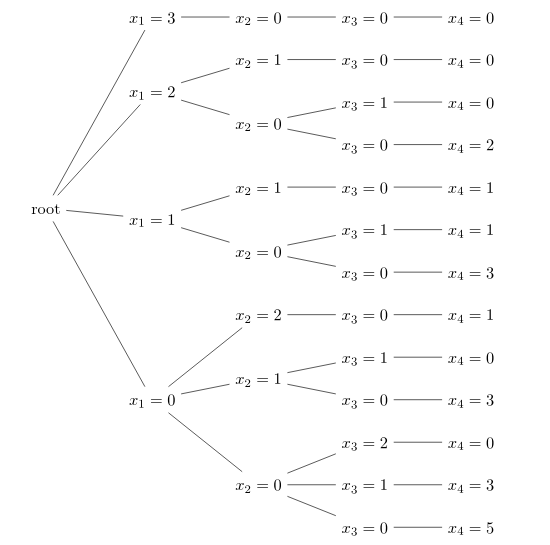
\includegraphics[width=\textwidth]{../image/chvatal_book_sample.png}
\caption{Drzewo wyliczeń możliwych rozwiązań} \label{fig:chvatalBBTree}
\end{figure}
drzewo będzie miało 13 liści (\cref{fig:chvatalBBTree}). Jeśli z jednego węzła wychodzi więcej niż jedna gałąź wówczas potomek o większej przechowywanej wartości jest umieszczany wyżej. Każdy następny węzeł jest obliczany według wzoru:
\begin{equation*}\label{eq:chvatalBBTree}
  \begin{aligned}
    & x_j = \lfloor{(c - \sum_{i=1}^{j-1}w_ix_i)/w_j}\rfloor \qquad i = 1,2,\dots,m \\
    & x_1 = \lfloor{c/w_1}\rfloor
  \end{aligned}
\end{equation*}
Drzewo (\cref{fig:chvatalBBTree}) jest drzewem po redukcji. Aby odrzucić węzły niepełniające warunków nierówności stosowany jest skrót: Poszukjąc rozwiązania $x_1,x_2,\dots,x_m$ ustawione zsotaje $k = m-1$. Jeśli zachodzi taka potrzeba zmienna $k$ jest dekrementowana dpóki nie zostanie znalezione $x_k > 0$. Wówczas $x_k = x_{k-1}$, a wartości $x_{k+1}, x_{k+2}, \dots,x_m$ są otrzymywane ze wzoru (\cref{eq:chvatalBBTree}).

Dla bieżącego rozwiązania $x_1^*,\dots,x_m^*$ zachodzi $\sum_{i=1}^m p_ix_i^* = M$. Maksymalne $k$ takie że $ k \le m - 1$ oraz $x_k > 0$ zostaje określone przechodząc od węzłów $x_1,x_2,\dots,x_m$ w stronę korzenia. Podobnie jak wcześniej niech $\bar{x}_i = x_i$ dla $i=1,2,\dots,k-1$ oraz $\bar{x}_k = x_k -1$ będą zmiennymi kandydującymi do rozwiązania. Aby okreslić czy $\bar{x_i}$ polepszy rozwiązanie $x_i^*$. Zgodnie z (\cref{eq:BBeff}) dla każdej zmiennej $x_{k+1}, x_{k+2}, \dots, x_m$ wydajność wynosi maksymalnie $p_{k+1}/w_{k+1}$, tak więc
\begin{equation*}
  \sum_{i=k+1}^m p_i\bar{x}_i \le {p_{k+1}}/{w_{k+1}}\sum_{i=k+1}^m w_i \bar{x}_i
\end{equation*}
połączone razem z (\cref{unboundedKnapsack}) zwraca:
\begin{equation}
  \sum_{i=1}^m p_i\bar{x}_i \le \sum_{i=1}^m w_i \bar{x}_i + {p_i}/{w_{i}}( c - \sum_{i=1}^k w_i\bar{x}_i ).
\end{equation}

\subsubsection{Programowanie dynamiczne}
Metoda ta używana jest w przypadku gdy problem można podzielić na małe podproblemy które można rozwiązać rekursywnie. Rozwiązanie optymalne podproblemu jest również optymalnym rozwiązaniem problemu głównego. Przedstawione zostanie rozwiązanie problemu plecakowego rodzaju 0-1 \cite{GoddardLecture}.

Jeśli elementy są oznaczone jako $1,\dots,n$ wtedy podproblem będzie odpowiedzialny za znalezienie optymalnego rozwiązania dla $S_k = \{1,2,\dots,k \}$. Niemożliwe jest opisanie rozwiązania końcowego $S_n$ na podstawie podproblemów $S_k$. Rekursywne sformułowanie podproblemu:
\begin{equation}\label{recursiveDynamic}
  \begin{aligned}
    B[k,w] =
    \begin{cases}
    & B[k-1,w] \quad \textrm{jeśli} \quad w_k > w, \\
    & max\{B[k-1,w], B[k-1,w-w_k] + b_k\} \quad \textrm{jeśli} \quad  w_k \le w.
    \end{cases}
  \end{aligned}
\end{equation}
Z powyższego równania wynika że najlepszy podzbiór podproblemu $S_k$ z całkowitą wagą $w$ jest najlepszym podzbiorem dla $S_{k-1}$ którego całkowita waga wymosi $w$ lub jest najlepszym podzbiorem dla $S_{k-1}$ którego całkowita waga wynosi $w-w_k$ plus $k$-ty element. Złożoność programowania dynamicznego to $O(n*W)$. Algorytm jako dane wejściowe przyjmuje maksymalną wartość ciężaru $W$, oraz dwie listy: listę wag $w_1,\dots,w_n$ oraz odpowiadającą jej listę zysku $b_1,\dots,b_n$.
\begin{algorithm}
  \caption{Programowanie dynamiczne - problem plecakowy 0-1}
  \begin{algorithmic}[1]
    \For {w := 0 TO W}
      \State B[0,w] := 0
    \EndFor
    \For {i := 1 TO n}
      \State B[i,0] := 0
    \EndFor
    \For {i := 1 TO n}
      \For {w := 0 TO W}
        \If {$w_i \le w$}
          \If {$b_i + B[i-1,w-w_i] > B[i-1,w]$}
            \State $B[i,w] := b_i + B[i-1,w-w_i]$
          \Else
            \State $B[i,w] := B[i-1,w]$
          \EndIf
        \Else
          \State $B[i,w] := B[i-1,w]$
        \EndIf
      \EndFor
    \EndFor
  \end{algorithmic}
\end{algorithm}
